% 
\documentclass[10pt]{article}
\usepackage{amscd,amsfonts,amssymb,amstext,latexsym} 
\usepackage{amsmath,mathbbol,mathrsfs,stmaryrd, mathtools} 
%\usepackage{mathbbol,mathrsfs,stmaryrd}
\usepackage {algorithm2e} 
\usepackage{theoremref}
\usepackage[T1]{fontenc}
\usepackage[english]{babel} 
\usepackage {enumerate}
\usepackage{url}
%\usepackage {algpseudocode}  
\usepackage{graphics} 
\usepackage{tikz}
\usepackage[square]{natbib}
\usepackage[]{geometry}
\usetikzlibrary{automata,calc}
%\usepackage{tgtermes} 
\usepackage{listings}
\usepackage{mathptmx}
\usepackage{fancyhdr}
\usepackage{verbatim}
\usepackage{enumitem}
\usepackage{booktabs}
\usepackage[flushleft]{threeparttable}
\usepackage{listings}
\usepackage{verbatim}
\usepackage{fancyhdr}
\usepackage{multirow,multicol}
\usepackage[colorlinks=true,linkcolor=blue,citecolor=blue,urlcolor=blue]{hyperref}
\usepackage{tabto}
\lstset{ %
language=C++,                % choose the language of the code
basicstyle={\ttfamily},       % the size of the fonts that are used for the code
backgroundcolor=\color{white},  % choose the background color. You must add \usepackage{color}
showspaces=false,               % show spaces adding particular underscores
aboveskip=6mm, 
%belowskip=3mm, 
numbers=left, numberfirstline=false, numberblanklines=false,
numberstyle=\tiny\color{gray}, numbersep= 5pt, 
showstringspaces=false,         % underline spaces within strings
showtabs=false,                 % show tabs within strings adding particular underscores
%frame=single,           % adds a frame around the code
%frame = tb, 
frame = none, 
tabsize=2,          % sets default tabsize to 2 spaces
captionpos=b,           % sets the caption-position to bottom
breaklines=true,        % sets automatic line breaking
breakatwhitespace=false,    % sets if automatic breaks should only happen at whitespace
escapeinside={\%*}{*)}          % if you want to add a comment within your code
}
%\graphicspath{{../../pics/}}
\fancypagestyle{plain}{
\fancyhf{}
\rhead{School of Computer Science and Applied Mathematics\\ 
%\noindent\rule{15.4cm}{0.4pt}\\
\footnotesize{\textsc{University of the Witwatersrand, Johannesburg}}}
\lhead{
\includegraphics[scale=0.08]{pics/witslogo_h.png}}
\fancyfoot[C]{\thepage}
\renewcommand{\headrulewidth}{0.4pt}
}

\textwidth=16.8cm 
\textheight=21.0cm 
\evensidemargin 0pt 
\oddsidemargin 0pt 
\leftmargin 0pt 
\rightmargin 0pt 
\setlength{\topmargin}{-20pt} 
\setlength{\footskip}{30pt}
\setlength{\parindent}{0pt}
\setlength{\parskip}{1em}
\linespread{1} 
% 
\makeatletter
\newcommand{\rmnum}[1]{\romannumeral #1}
\newcommand{\Rmnum}[1]{\expandafter\@slowromancap\romannumeral #1@}
\makeatother


\begin{document}
\title{COMS3008A Assignment One -- Report}
\author{Put your name, student number here}
\date{Put your submission date here} 
\maketitle 
%\thispagestyle{empty}
\pagestyle{fancy}
\fancyhf{}
\fancyhead[R]{\thepage}
\fancyhead[L]{COMS3008A Assinment}
%\vskip 3mm 
%\pagenumbering{roman}
%\newpage
\pagenumbering{arabic} 
\section{Problem 1: Parallel Scan}
\begin{itemize}
	\item  Given a set of elements, $[a_0,a_1,\dotsm,a_{n-1}]$, the scan operation associated with addition operator for this input is the output set $[a_0,(a_0+a_1),\dotsm,(a_0+a_1+\dotsm+a_{n-1})]$. 
	\item For example, the input set is $[2,1,4,0,3,7,6,3]$, then the scan with addition operator of this input is $[2,3,7,7,10,17,23,26]$. 
\end{itemize}

\section{Problem 2: Parallel Bitonic Sort}
The bitonic sort is based on the idea of sorting network. The bitonic sorting algorithm is suitable for parallel processing, especially for GPU sorting. \textbf{However, in this problem, you are requested to implement parallel bitonic sorting of integers using \textbf{OpenMP and MPI}, respectively. }

Another paragraph starts \dots
\section{Problem 3: Parallel Graph Algorithm}
An example figure is given in Figure~\ref{fig:sp_fig1}.
\begin{figure}[htb]
	\centering
	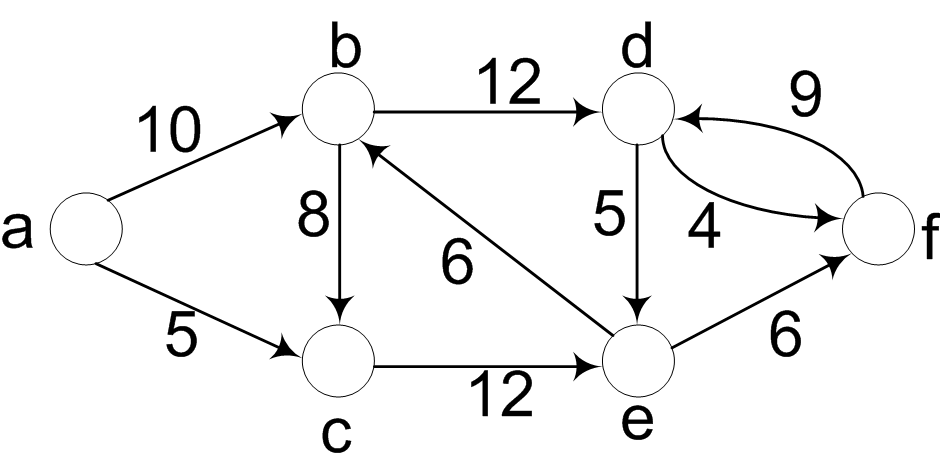
\includegraphics[width=0.5\linewidth]{pics/sp_fig1.png}
	\caption{A directed graph}\label{fig:sp_fig1}
\end{figure}

An example of table is given Table~\ref{tab:example}.
\begin{table}[htb]
	\centering
	\caption{An example of a table}\label{tab:example}
	\begin{tabular}{l|ccccc}
		\toprule
		No of vertices & 64 & 128 & 256 & 384 & 512\\
		\midrule
		Serial &0.1&0.2&0.3&0.4&0.5\\
		Parallel &&&&\\
		Sppedup &2&3&4&5&6\\
		\bottomrule
	\end{tabular}
\end{table} 

\end{document} 




